\noindent As mentioned in the Chapter \ref{Lspec}, the distance between the CEC and the LCR introduces the possibility of optical pumping, a process that changes the ground state distribution of the atoms as they travel the distance between the two regions. This change in ground state distribution is induced by the interaction of the atoms with the laser before they reach the LCR. In an atomic system that has not interacted with a laser, the ground state distribution of the hyperfine levels is statistical.\cite{townsend} The likelihood of an electron occupying hyperfine level \textbf{F} is proportional to $2F+1$. In a system with N hyperfine ground states, each with \textbf{F} = \textbf{F}$_n$, where $n$ = 1,2,3,..N, the probability of an electron occupying, the $i$-th level is given by \cite{townsend}
\begin{equation}
\mathrm{Prob(F}_i) = \frac{2F_i+1}{\sum_{j=1}^\mathrm{N}2F_j+1}.
\end{equation}
However, as the electron goes through a series of excitation/decay cycles, certain ground states will be selected over others, depending on selection rules as well as transition probabilities. Optical pumping manifests itself through the modification of the relative peak heights in a hyperfine spectrum, as shown in Fig. \ref{OP_francium}, where the peak heights of a hyperfine spectrum of Francium show the effects of optical pumping. The expected peak heights as calculated by the Racah intensities are shown in red, and are compared to the intensities measured with the laser continuously on (solid black) and those measured when the laser was pulsed (black outline). The pulsed intensities are similar to the expected intensities, while those measured with a continuous wave (cw) laser deviate significantly.
\begin{figure}[h]
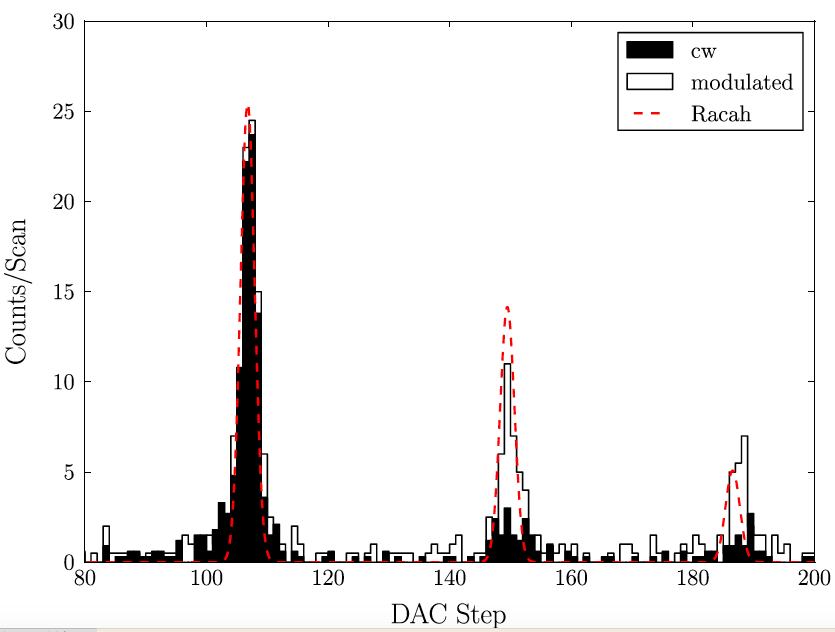
\includegraphics[width=\textwidth]{Graphics/francium.png}
\caption[Demonstration of the effects of optical pumping on the relative peak heights for a hyperfine spectrum of Francium-208.]{\small Demonstration of the effects of optical pumping on the relative peak heights for a hyperfine spectrum of Francium-208. The Racah intensities are shown in red, while the intensities measured for a continuous wave (cw) laser and a pulsed laser are shown in solid black and black lines, respectively. The Digital Analogue Converter (DAC) is proportional to the laser frequency. The cw measurements deviate significantly from the Racah intensities, while the pulsed measurements are closer to the expected intensities\cite{CFBS}.}
\label{OP_francium}
\end{figure}

To illustrate the effect of mechanisms of optical pumping, consider the following: A hyperfine system has two ground states, $\bf{F}_1$ and $\bf{F}_2$, as well as an excited state $\bf{F}_3$, as shown in Fig. \ref{toy_model}.
\begin{figure}[h]
\begin{center}
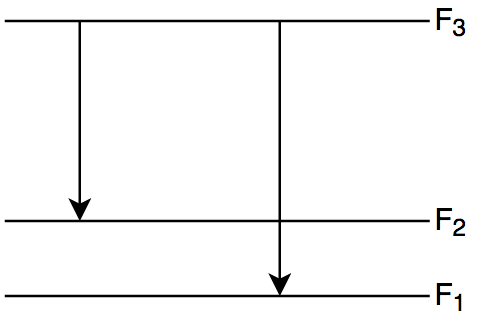
\includegraphics[width=\textwidth]{Graphics/Toy_model.png}
\caption[Toy model of a hyperfine system with two ground states.]{\small Toy model of a hyperfine system with two ground states, $\bf{F}_1$ and $\bf{F}_2$, and a single excited state $\bf{F}_3$. If this system is exposed to a laser resonant with the $\bf{F}_2 \rightarrow \bf{F}_3$ transition, then as the atom goes through excitation and decay cycles, the chances of having an electron in $\bf{F}_2$ available for excitation decrease.}
\label{toy_model}
\end{center}
\end{figure}
When the atom is in the excited state, it has probability $P(\bf{F}_3 \rightarrow \bf{F}_2)$ of decaying to the $\bf{F}_2$ state, and probability $1-P(\bf{F}_3 \rightarrow \bf{F}_2)$ of decaying to the $\bf{F}_1$ state. If the atom is exposed to a laser resonant with the $\bf{F}_2 \rightarrow \bf{F}_3$ transition, what is the probability that after time $t$ the ground state of the atom is still $\bf{F}_2$? Say that the lifetime of the $\bf{F}_2 \rightarrow \bf{F}_3$ transition is $\tau$, and that the average time for a resonant photon to be absorbed is $t_{\mathrm{abs}}$. Then the number of excitation/decay cycles in time $t$, $N_{\mathrm{cycles}}$, is
\begin{equation}
N_{\mathrm{cycles}}=\frac{t}{\tau+t_{\mathrm{abs}}}.
\end{equation}
rounded down to the closest integer. If at any time, the atom decays to the $\bf{F}_1$ state, then it is no longer on resonance and the chances of a photon being absorbed are negligible. As such, the probability that the atom is in $\bf{F}_2$ after $\mathrm{\bf{N}}_{\mathrm{cycles}}$ is
\begin{equation}
P(\bf{F}_2) = P(\bf{F}_3 \rightarrow \bf{F}_2)^{\mathrm{\bf{N}}_{\mathrm{cycles}}}.
\end{equation}
As $P(\bf{F}_3 \rightarrow \bf{F}_2) < 1$, then the chances of finding an electron in the $\bf{F}_2$ state decrease as $t$ increases. If, for example, one began measuring the number of resonant photons emitted after time $t$ for a collection of atoms with the above hyperfine structure, the number of photons measured would be reduced by a factor of $P(\bf{F}_2)$. This calculation is the basis for the method used in this work to measure the effect of optical pumping on the atoms being investigated at the CFBS, presented in the following section.

\section{Optical Pumping as a Modification to the Racah Intensities}
To evaluate the effects of optical pumping on a hyperfine spectrum collected at the CFBS experiment, the toy model presented above need only be expanded on. The important quantities are the time an atom interacts with the laser before entering the LCR, the time it takes for a resonant photon to be absorbed, the lifetimes of each excited state and the probability of an electron decaying to the ground state from which it originated. The computation of each of these quantities is shown in this section, after which they are combined to calculate how the Racah intensity for each transition must be modified to show the effects of optical pumping.

\subsection{Interaction Time}
The interaction time, $t_{\mathrm{int}}$ is the time that the atom will be possibly be interacting with the laser before entering the LCR. Its calculation is straightforward. If the distance between the CEC and the LCR is $d$, and the atoms are moving at a velocity $v$, then the interaction time is
\begin{equation}
t_{\mathrm{int}} = \frac{d}{v}.
\end{equation}
While $d$ is a static quantity, $v$ changes depending on the frequency of the laser and the resonant frequency of the transition in question. As mentioned in Chapter \ref{Lspec}, the CFBS fixes the frequency of the laser and uses electrodes to alter the speed of the oncoming atoms, shifting the frequency observed by the atoms. Knowing the initial energy of the beam $E_b$ and the mass of the atoms $m_A$, the initial velocity of the atoms is 
\begin{equation}
v_{\mathrm{init}}=\sqrt{\frac{2E_b}{m_A}},
\end{equation}
If the resonant frequency of a transition is $f_{\mathrm{res}}$ and the frequency of the laser is $f_{\mathrm{las}}$, then the velocity at which the atom will observe $f_{\mathrm{res}}$, $v_{\mathrm{res}}$, is described by \cite{cmec}
\begin{equation}
f_{\mathrm{res}} = f_{\mathrm{las}} \sqrt{\frac{1+v_{\mathrm{res}}/c}{1-v_{\mathrm{res}}/c}}.
\end{equation}
Rearranging yields the following expression for $v_{\mathrm{res}}$
\begin{equation}
v_{\mathrm{res}} = c \frac{(f_{\mathrm{res}}/f_{\mathrm{las}})^2-1}{(f_{\mathrm{res}}/f_{\mathrm{las}})^2+1}
\end{equation}
and
\begin{equation}
t_{\mathrm{int}} = \frac{d}{c} \frac{(f_{\mathrm{res}}/f_{\mathrm{las}})^2+1}{(f_{\mathrm{res}}/f_{\mathrm{las}})^2-1}
\end{equation}

\subsection{Absorption Time of a Resonant Photon}
For a chosen transition, what is the expected time, $t_{\mathrm{abs}}$ that passes before a resonant photon is absorbed by the atom, given a laser field of intensity $I$? This is simply the inverse of the scattering rate, as described in Eq. \ref{scatt_rate}, evaluated at resonance, i.e. $\delta = 0$
\begin{equation}
t_{\mathrm{abs}} = \left(\frac{s_0\gamma/2}{1+s_0}\right)^{-1}.
\end{equation}

\subsection{Lifetime of an Excited State}
This quantity is already known. The inverse of Eq. \ref{gamma} gives the lifetime, $\tau$, of a particular transition
\begin{equation}
\tau = \frac{3\pi\epsilon_0\hbar c^3}{\omega^3\mu^2}.
\end{equation}

\subsection{Time for Excitation/Decay Cycle}
Combining the results from the two above sections, the average time that it takes for an atom to go through an excitation/decay cycle, assuming that it returns to the ground state that it was in before excitation, $t_{\mathrm{cycle}}$, is
\begin{align}
t_{\mathrm{cycle}} =& t_{\mathrm{abs}}+ \tau\\
=& \left(\frac{s_0\gamma/2}{1+s_0}\right)^{-1} + \frac{3\pi\epsilon_0\hbar c^3}{\omega^3\mu^2}
\end{align}

\subsection{Probability of Returning to Original Ground State}
\label{pogs}
The probability of an atom decaying to the ground state from which it was excited is computed by comparing the decay rates of all possible transitions that share the same excited state as the transition in question, i.e., 
\begin{equation}
P(\mathrm{OGS}) = \frac{\gamma_{\mathrm{OGS}}}{\sum_{\mathrm{PT}}\gamma_{\mathrm{PT}}}
\end{equation}
where $P(\mathrm{OGS})$ is the probability of the atom returning to the original ground state, $\gamma_{\mathrm{OGS}}$ is the decay rate of the transition that results in the return to the original ground state and $\gamma_{\mathrm{PT}}$ is the decay rate of all possible transitions that share the same excited state as the transition in question.

\subsection{Probability of Reaching the LCR}
\label{pogslcr}
Finally, the probability of an atom reaching the LCR without changing its ground state is given by
\begin{equation}
P(\mathrm{OGS\ at\ LCR}) = \left(\frac{\gamma_{\mathrm{OGS}}}{\sum_{\mathrm{PT}}\gamma_{\mathrm{PT}}}\right)^{\frac{t_{\mathrm{int}}}{t_{\mathrm{cycle}}}}
\label{prob_unchanged}
\end{equation}
where $\frac{t_{\mathrm{int}}}{t_{\mathrm{cycle}}}$ is rounded down to the nearest integer, reflecting the fact the excitation/decay cycles are quantized events.

\section{Modification of the Racah Intensities}
Now that the probability of finding an atom in its original ground state when it reaches the LCR is known, the effects of optical pumping can be simulated through the modification of the Racah intensity for each transition. For a given transition $\bf{F}_e \rightarrow \bf{F}_g$ the modified Racah intensity, $I_{R_{\mathrm{mod}}}$, is 
\begin{align}
I_{R_{\mathrm{mod}}} =& P(\mathbf{F}_g\ \mathrm{at\ LCR})
(2F_e+1)(2F_g+1)
\left\lbrace
\mathrm{
\begin{matrix}
F_g & F_e & 1\\
J_e & J_g & \mathrm{I} 
\end{matrix}
}
\right\rbrace^2\\
=& \left(\frac{\gamma_{\mathrm{OGS}}}{\sum_{\mathrm{PT}}\gamma_{\mathrm{PT}}}\right)^{\frac{t_{\mathrm{int}}}{t_{\mathrm{cycle}}}}
(2F_e+1)(2F_g+1)
\left\lbrace
\mathrm{
\begin{matrix}
F_g & F_e & 1\\
J_e & J_g & \mathrm{I} 
\end{matrix}
}
\right\rbrace^2
\label{final_eq}
\end{align}
which results from the combination of Equations \ref{prob_unchanged} and \ref{RACAH}.

\section{Summary}
In this Chapter, optical pumping was treated as a modification to the Racah intensities, which describe the intensities of hyperfine transitions. Optical pumping changes the ground state distribution of the atoms/ions before they enter the LCR. To simulate this effect, the probability of an atom reaching the LCR the without changing ground state was calculated (Sections \ref{pogs} and \ref{pogslcr}) for each hyperfine transition. This probability was a function of the laser power, the distance between the CEC and the LCR, and the likelihood of the transition in question. Once the probability of an atom remaining in its original ground was known, the corresponding Racah intensity was multiplied to get the adjusted intensity for that particular transition. 

\subsection{Previous Method: Monte-Carlo Type Simulation}
The method developed above is based on statistical ensembles describing the state of the atoms/ions as they pass through the experiment. Previously, a full simulation of each atom as it passed through the experiment was developed. This method was eventually abandoned due to the excessive computation time required. For posterity's sake, it is mentioned here.


In this section, the Monte-Carlo simulation of a hyperfine spectrum measured at TRIUMF is described in detail. $\S$\ref{pip} includes little more than a graphical representation of the algorithm followed when the atoms are interacting with the laser. Each subsequent section is dedicated to an individual step in the algorithm, detailing the logic and computations required at that step. The final section shows how a hyperfine spectrum is built through the repeated application of the interaction loop.

\begin{figure}[h]

\begin{tikzpicture}[node distance = 2.5cm]
\tiny

\node (props) [prelim] {Select velocity and ground state};
\node (exprobs) [prelim, right of=props] {Compute exitation rates};
\node (Adv_exc) [block, right of=exprobs] {Advance by eaxcitation time};
\node (IR) [decision, above of=Adv_exc] {In IR?};
\node (Exc) [block, right of=IR] {Excite to new state};
\node (Adv_life) [block, right of=Exc] {Advance by mean lifetime};
\node (IR_2) [decision, below of=Adv_life] {In IR?};
\node (Next) [end, right of=IR_2] {Next atom};
\node (deex) [block, below of=IR_2] {Deexcite and select new ground state};
\node (LCR) [decision, left of=deex] {In LCR?};
\node (PHO) [block, left of=LCR] {Record photon and increase counter};
\node[coordinate] (bl1) [above of = IR,yshift=-15mm]{};
\node[coordinate] (bl2) [above of=Next]{};
\node[coordinate] (bl3) [above of=bl2,yshift=-15mm]{};
\node[coordinate] (bl4) [above of = LCR,yshift = -15mm]{};
\node[coordinate] (bl5) [left of =PHO,yshift = 5mm]{};

\draw [arrow] (props)--(exprobs);
\draw [arrow] (exprobs)--(Adv_exc);
\draw [arrow] (Adv_exc)--(IR);
\draw [arrow] (IR) -- node[anchor=south] {Yes} (Exc);
\draw (IR) -- node[anchor=north east,yshift = 1mm] {No} (bl1);
\draw (bl3) -- (bl1);
\draw [arrow] (bl3)--(Next);
\draw [arrow] (Exc)--(Adv_life);
\draw [arrow] (Adv_life) -- (IR_2);
\draw [arrow] (IR_2) -- node[anchor = south] {No} (Next);
\draw [arrow] (IR_2) -- node[anchor = east] {Yes} (deex);
\draw [arrow] (deex) -- (LCR);
\draw [arrow] (LCR) -- node[anchor = south] {Yes} (PHO);
\draw (LCR)-- node[anchor = west] {No} (bl4);
\draw [arrow] (PHO) -| (exprobs);
\draw [arrow] (bl4)-|(exprobs);
\end{tikzpicture}
\caption[Flow chart detailing the steps undertaken by the alternative algorithm to follow the atom as it moves through the IR.]{\small Flow chart detailing the steps undertaken by the algorithm to follow the atom as it moves through the IR. The green ellipses and blue rectangles compose the interaction loop of the simulation, where the atom interacts with the laser and goes through excitation/decay cycles. Finally, the yellow rectangle is the end point of the loop, and occurs when then atom has moved beyond the IR.}
\label{pipeline}
\end{figure}

\label{pip}


\section{Interaction Loop}


Fig. \ref{pipeline} shows each step taken an atom as it passes through the simulation. The red rounded rectangles represent preliminary steps in the simulation, where initial properties are imparted to the atom. The first preliminary step selects a velocity and ground state for the atom. The following step is the calculation of the likelihood of excitation for each allowed transition. This prepares the atom for what can be considered the main loop of the algorithm. Here, the atom and laser interact as the atom traverses the IR. 

The interaction loop is composed of green ellipses and blue rectangles. Two of the three green ellipses represent regular checks to ensure that the atom is still in the IR. If at any point the atom is found to have moved beyond the IR, then the algorithm moves on to the next atom. The third green ellipse is dedicated to checking if a photon released by the atom would be measured by the PMT. The evolution of the state and position of the atom is described by the blue rectangles. 

\subsection{Preliminary Steps}
The first two steps select the initial properties given to the atom, determining how likely the atom is to interact with the laser. The two most important properties are the velocity and the ground state of the atom. Both are chosen through the sampling of their respective probability distributions.

\subsubsection{Velocity Selection}

The velocity of the atom $v_a$ can be decomposed in to two elements: the mean velocity of the beam, $v_{m}$, and the thermal velocity $v_{T}$. 
\begin{equation}
v_a = v_m + v_T
\end{equation}
The mean velocity is determined by the energy of the beam and the mass of the atom, i.e.
\begin{equation}
v_{m} = \sqrt{\frac{2E_b}{m_A}}
\end{equation}
where $E_b$ is the energy of the beam and $m_A$ is the mass of an atom with mass number $A$.

The thermal velocity is selected by sampling the Maxwell-Boltzmann distribution (Eq. \ref{MBD}). This is done using the Box-Muller transform, which samples a uniform distribution twice and converts the results into a sample of a normal distribution. A sample $v_T$, of a Maxwell-Boltzmann distribution
\begin{equation}
v_T = \sigma_{MB} \sqrt{-2\log x_1}\cos (2\pi x_2)
\end{equation}
where $x_1,x_2 \in [0,1]$ are two randomly generated numbers taken from a uniform distribution and $\sigma_{MB}$ is the square root of the variance of the Maxwell-Boltzmann distribution. 

\subsubsection{Ground State Selection}
For an atom with a coupled angular momentum state $F_g$ as the ground state, the electron can occupy any of the $2F_g+1$ projections on the axis of quantization. A particular projection, say $F_i \in [-F_g,-F_g+1,...,F_g-1,F_g]$, has a probability of being occupied that is proportional to $2F_i+1$. Taking the probability space occupied by each projection in to account, the probability that an electron occupies the projection $F_i$, $P(F_i)$, is given by
\begin{equation}
P(F_i) = \frac{2F_i+1}{\sum_j 2F_j+1}
\label{gs_prob}
\end{equation}
Knowing this, the ground state can be chosen through the generation of a random number $x \in [0,1]$ from a uniform distribution. Each projection is given a range of numbers from 0 to 1, proportional to Eq. \ref{gs_prob}. If $x$ falls in the assigned range, then that ground state is chosen. 

\subsubsection{Computation of Excitation Rates}
With the ground state and the velocity of the atom now selected, the probability that a transition will occur can be calculated. For each allowed transition between the chosen ground state $F_g$ and an excited state $F_{e,i}$, the transition rate $\gamma_i$ is given by Eq. \ref{scatt_rate}. Note that the laser frequency $f_l$ must be shifted according to Eq. \ref{dop_shift}.

\subsection{Interaction Loop}
The interaction loop of the algorithm is the place where the atoms undergo several instances of excitation and decay. Also included are regular checks to see in the atom would still be present in the in interaction region, as well as whether or not a released photon would be measured by the light collection system present in the experiment.

\subsubsection{Excitation Time}
Once all the excitation rates have been computed, the atom can now be advanced by the expected time it takes for a transition to occur. This time is called the excitation time, $t_e$, and is given by
\begin{equation}
t_e = \sum_i \frac{1}{\gamma_i}
\end{equation}
After time $t_e$, the atom is advanced a distance $d_e = t_ev_a$. If it is still in the interaction region, then an excited state $F_e$ is chosen by sampling a uniform distribution where each transition is given a region proportional to $1/\gamma_i$, in similar style to the method used to select the ground state. If the atom is no longer in the interaction region after $t_e$, then it is discarded and the algorithm moves on to the next atom.

\subsubsection{Advancing by the Mean Lifetime, Decay and Selection of New Ground State}
Once the excited stated of the atom has been selected, then the atom is advanced a distance $d_l = t_lv_a$ where $t_l$ is the mean lifetime of the excited state. The mean lifetimes of each excited state are computed (according to $\S$ \ref{ALI}) once at the beginning of the simulation, then stored for later use. If the atom is still in the interaction region after having moved $d_l$, then it decays into one of the allowed ground states. If not, then the simulation moves on to the next atom. As with the selection of the excited state, a uniform distribution is sampled, and each ground state $F_{g,i}$ is given a range of values proportional to the inverse of the lifetime of the transition from the excited state, $F_{e}$, to $F_{g,i}$. 

Once a ground state is selected, a photon with energy given by Eq. \ref{HFE} is "released". If the atom is in the light collection region, then this photon is recorded for later analysis. Additionally, a counter that keeps track of the number of photons collected at each beam energy is increased by one. If the atom is not in the LCR, then nothing is recorded, and the excitation-decay process begins again with the computation of excitation rates.

\subsection{Simulation of Complete Run}
In order to simulate a complete experimental run, a chosen number of atoms, say N, are passed in sequence through the above loop. This is done in turn for each beam energy in a list of energies that are selected such that the Doppler shifted laser energies range from the lowest energy to the highest energy transition, with some leeway on either side. This range can be called $E_r$. The graph of photon counts per beam energy is in fact the hyperfine spectrum. Alg. \ref{alg} shows the pseudo-code that is followed for the simulation of a collection of atoms passing through the experiment. Following Alg. \ref{alg} is a list of all the preliminary parameters needed by the simulation in order to compute the necessary quantities presented in this section. 

\vspace{10mm}
\begin{algorithm}[H]
\SetAlgoLined
\KwResult{Simulation of complete hyperfine spectrum}
 Input all preliminary parameters\;
 \For{Beam energy in $E_r$}{
  \For{Each atom}{
   Run \textbf{interaction loop}\;
   Record photon count\;
  }
  Sum photon count into counts per beam energy\;
 }
 Plot photon count at each beam energy\;
 \caption{Pseudo-code for the simulation of a complete hyperfine spectrum.}
 \label{alg}
\end{algorithm}

\vspace{10mm}
The preliminary parameters mentioned in the above pseudo-code refer to all the quantities required to perform a complete simulation of a hyperfine spectrum measured at TRIUMF. A list of these parameters is provided below, for completeness.

\begin{list}{•}{List of Preliminary Parameters and Their Symbols}
\item Isotope mass: $m_A$
\item Ground J-state: $\bf{J}_g$
\item Excited J-state: $\bf{J}_e$
\item Nuclear spin: $\bf{I}$
\item Principal quantum number of ground state: $n_g$
\item Principal quantum number of excited state: $n_e$
\item Magnetic dipole hyperfine coefficient of ground state: $A_g$
\item Magnetic dipole hyperfine coefficient of excited state: $A_e$
\item Electric quadrupole hyperfine coefficient of ground state: $B_g$
\item Electric quadrupole hyperfine coefficient of excited state: $B_e$
\item Beam temperature: $T_b$
\item Laser frequency: $f_l$
\item Laser intensity: $I_l$
\item Fine structure transition energy: $E_{fs}$
\item Number of atoms to simulate per beam energy: $N_a$
\item Distance between CEC and LCR: $d$
\item Length of LCR: $d_{LCR}$
\end{list}